\documentclass[a4paper,11pt]{ltjsarticle}
\usepackage{base}
\title{}
\author{}
\date{}
\newcommand{\printheader}[2]{
\begin{tikzpicture}[remember picture, overlay]
\node[yshift=-2.5cm, anchor=north] at (current page.north) {
\begin{tikzpicture}
\fill[gray!20] (0,0) rectangle (\textwidth, 2cm);
\fill[gray!80] (0,0) rectangle (0.2cm, 2cm);
\draw[gray!80, thick] (0,0) -- (	\textwidth, 0);
\node[anchor=west, text width=\textwidth-1cm, inner xsep=1cm] at (0, 1.25cm) {
\parbox[b]{\linewidth}{
{\color{gray!50!black}\bfseries #1} \par
\vspace{0.2em}
{\huge\bfseries #2}
}
};
\end{tikzpicture}
};
\end{tikzpicture}
\vspace{0.5cm}
}
\begin{document}
\printheader{単元別演習 2次関数①}{最大・最小}
\begin{exque}
     2次関数$y=-x^2+2ax-a^2+3~(-1\leqq x\leqq1)$の最大値を求めよ.また,そのときの$x$を求めよ.
\end{exque}
\ascboxG{\textbf{Point.}}文字定数を含む関数の最大・最小→グラフを描いて場合分け!
\ans 
 まず,平方完成をすると$-x^2+2ax-a^2+3=-(x-a)^2+3$であるから,グラフは$(a,3)$を頂点とする上に凸の放物線である.頂点と定義域の位置関係によって場合分けする.

    \begin{itemize}
        \item [(1)]$a<-1$のとき,区間の左端で最大値をとることがわかる.よって,$\boldsymbol{x=-1}$で最大値$\boldsymbol{-a^2-2a+2}$.
     \item [(2)]$-1\leqq a\leqq 1$のとき,頂点が定義域内に入るので,頂点で最大値をとることがわかる.よって,$\boldsymbol{x=a}$で最大値$\boldsymbol{3}$.
  
        \item [(3)]$a>1$のとき,区間の右端で最大値をとることがわかる.よって,$\boldsymbol{x=1}$で最大値$\boldsymbol{-a^2+2a+2}$.

        \end{itemize}
        \begin{minipage}{0.33\linewidth}
     \begin{figure}[H]
            \centering
            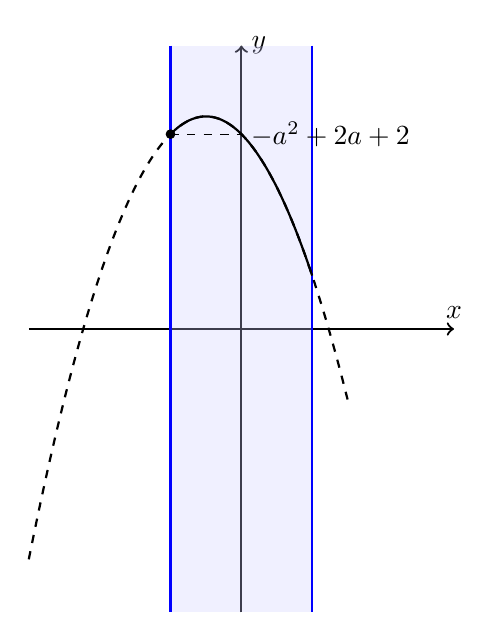
\begin{tikzpicture}[scale=0.9]
                \draw[thick,->](-3,0)--(3,0)node[above]{$x$};
                \draw[thick,->](0,-4)--(0,4)node[right]{$y$};
                \fill[blue!20,opacity=0.3] (-1,-4) rectangle (1,4);
                \draw[thick,blue](1,4)--(1,-4);
                \draw[thick,blue](-1,4)--(-1,-4);
                   \draw[domain=-1:1 ,samples=100, smooth,thick] plot (\x, {-\x*\x-\x+2.75}); 
                   \draw[dashed,domain=-3:1.5 ,samples=100, smooth,thick] plot (\x, {-\x*\x-\x+2.75}); 
                   \draw[fill=black](-1,2.75)circle[radius=0.06];
                   \draw[dashed](-1,2.75)--(0,2.75)node[right]{$-a^2+2a+2$};
            \end{tikzpicture}
            \end{figure}
        \end{minipage}
        \begin{minipage}{0.33\linewidth}
               \begin{figure}[H]
            \centering
            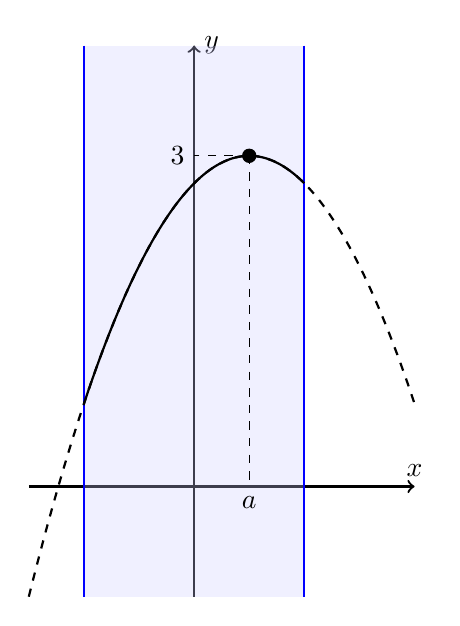
\begin{tikzpicture}[scale=1.4]
                 \draw[thick,->](-1.5,0)--(2,0)node[above]{$x$};
                 \draw[thick,->](0,-1)--(0,4)node[right]{$y$};
                 \fill[blue!20,opacity=0.3] (-1,-1) rectangle (1,4);
                 \draw[thick,blue](1,4)--(1,-1);
                 \draw[thick,blue](-1,4)--(-1,-1);
                   \draw[domain=-1:1 ,samples=100, smooth,thick] plot (\x, {-\x*\x+\x+2.75}); 
                   \draw[dashed,domain=-1.5:2 ,samples=100, smooth,thick] plot (\x, {-\x*\x+\x+2.75}); 
                   \draw[fill=black](0.5,3)circle[radius=0.06];
                   \draw[dashed](0.5,3)--(0,3)node[left]{3};
                   \draw[dashed](0.5,3)--(0.5,0)node[below]{$a$};
            \end{tikzpicture}
            \end{figure}
        \end{minipage}
               \begin{minipage}{0.33\linewidth}
           \begin{figure}[H]
            \centering
            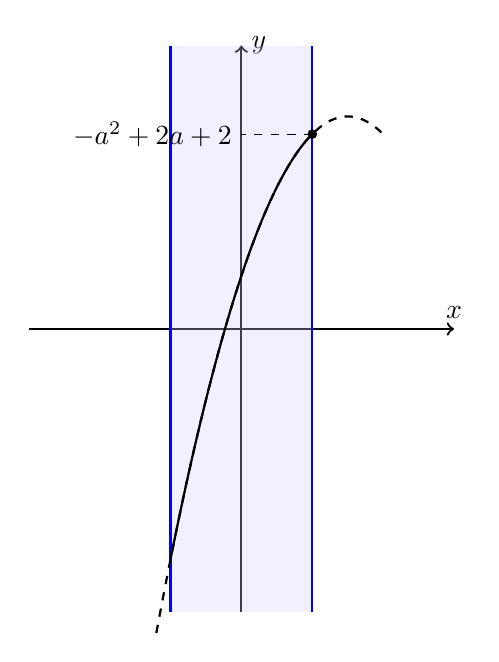
\begin{tikzpicture}[scale=0.9]
                \draw[thick,->](-3,0)--(3,0)node[above]{$x$};
                \draw[thick,->](0,-4)--(0,4)node[right]{$y$};
                \fill[blue!20,opacity=0.3] (-1,-4) rectangle (1,4);
                \draw[thick,blue](1,4)--(1,-4);
                \draw[thick,blue](-1,4)--(-1,-4);
                   \draw[domain=-1:1 ,samples=100, smooth,thick] plot (\x, {-\x*\x+3*\x+0.75}); 
                   \draw[dashed,domain=-1.2:2 ,samples=100, smooth,thick] plot (\x, {-\x*\x+3*\x+0.75}); 
                   \draw[fill=black](1,2.75)circle[radius=0.06];
                   \draw[dashed](1,2.75)--(0,2.75)node[left]{$-a^2+2a+2$};
            \end{tikzpicture}
            \end{figure}
        \end{minipage}
        \begin{toi}
        $a$ を負の定数とする。2次関数 $f(x) = ax^2 - 2ax + b$ の $-2 \le x \le 2$ における最大値が $12$, 最小値が $-6$ のとき、$a, b$ の値を求めよ。
\hfill [04 同志社女子大]
        \end{toi}
\begin{exque}
$x$を実数とする.$A = x^2 - 2x$ とおくとき,$A$の最小値は~\fbox{ ア }~である.したがって、$y=(x^2 - 2x)^2 + 4(x^2 - 2x)$ の最小値は~\fbox{ イ }~である.
\hfill [07 北海道工大]
\end{exque}
\ascboxG{\textbf{Point.}}変数の置き換え→範囲に注意!
\ans 
$A=(x-1)^2-1$であるから,$A$は$x=1$で最小値$\boldsymbol{-1}$をとる.$\cdots \fbox{ ア }$\\
 よって,$A\geqq -1$であるから,$y=(x^2 - 2x)^2 + 4(x^2 - 2x)=A^2+4A~(A\geqq-1)$の最小値を求めればよい.$y=(A+2)^2-4$なので,$A=-1$で最小値$-3$をとる.$\cdots \fbox{ イ }$\
\begin{toi}
関数 $y = (x^2 -3x)^2 -9(x^2 -3x) ~(1\leqq x\leqq4)$ の最大値と最小値を求めよ.\hfill [05 慶應義塾大]
\end{toi}
 \\
\ascboxA{\textbf{復習問題}}
\begin{toi}
関数 $y =-2\sin^2x + 5\sin x +3~(0\leqq x\leqq 2\pi)$ の最小値を求めよ.
\end{toi}
\begin{toi}
$0 \le x \le 3$ のとき、関数 $f(x) = 2x^2 - 4ax + a + a^2$ の最小値 $m$ が $0$ となるような定数 $a$ の値をすべて求めよ。
\hfill [86 東京大]
\end{toi}
\begin{toi}
2次関数$f(x)=ax^2-6ax+b$は,区間$1\leqq x\leqq4$において最大値11,最小値8をとる.このとき,$a>0$ならば,$b=~\fbox{ ア }$であり,$a<0$ならば,$b=\fbox{ イ }$である.\hfill{[06 愛知工業大]}
\end{toi}
\end{document}